% La conclusión debe contener los principales aspectos y contribuciones para finalizar el trabajo presentado. Se debe presentar lo que se esperaba del trabajo a través de los objetivos introducidos inicialmente y mostrar lo que se logró. No se debe insertar un nuevo asunto en la conclusión. Aquí el autor presentará las propias impresiones sobre el trabajo efectuado. Es importante también que se identifiquen limitaciones y problemas que surgieron durante el desarrollo del trabajo y cuáles las consecuencias del mismo.

% Los trabajos futuros deben contener oportunidades de expansión del trabajo presentado, así como nuevos proyectos que pudieron ser vislumbrados a partir del desarrollo del trabajo.

\chapter{Conclusiones y Trabajo Futuro}
\label{ch:Conclusiones y Trabajo Futuro}

\begin{quote}
  {\bf\textsc{Resumen:}} Este capítulo recoge los principales aspectos y contribuciones obtenidos para la integración de Información Geográfica en la Web Semántica. De igual manera, comprobaremos el cumplimiento de los objetivos que introducimos inicialmente en el \texttt{Capítulo 1}. Asimismo, se comentarán posibles propuestas de mejora de cara a sucesivas iteraciones del proyecto, además de comentar otras posibles aplicaciones empleadas, que caen fuera del ámbito de este trabajo.
\end{quote}




\section{Conclusiones}

En este TFM se ha profundizado ... \\


Por tanto, mediante el desarrollo de este TFM, considero que se han conseguido los objetivos señalados en el capítulo 1, en concreto:


Dos áreas distintas  y las estoy aplicando conjuntamente.

\begin{enumerate}
	
	\item \textbf{Comprender la relación existente entre los Sistemas de Información Geográfica y la Web Semántica}, a priori dos áreas completamente diferentes.
	
	\item \textbf{Hacer uso de fuentes de información geoespacial}, con las que obtener datos públicos geográficos de buena calidad.
	
	\item \textbf{Localizar diversas herramientas de la Web Semántica} que se puedan utilizar para representar e integrar Información Geográfica.
	
	\item Aprender a \textbf{agregar conocimiento de dominio geoespacial sobre la estructura de los datos} mediante el empleo de herramientas de la Web Semántica como Protegé.
	
	\item \textbf{Aprender a crear ontologías y poblarlas}  mediante información geográfica existente.
	
	\item Apreciar las carencias o mejoras que supone usar \textbf{Protegé frente a otro tipo de herramientas}.
	
	\item Conocer cuál es la \textbf{estructura de los datos geoespaciales y sus especificaciones para realizar consultas con el lenguaje GeoSPARQL}.
	
	\item Aprender a \textbf{ubicar información geoespacial en un mapa mediante el uso de la biblioteca Leaflet}.
	
	\item Mostrar algunos \textbf{métodos de trabajo}, estrechamente adaptados al tratamiento de Información Geográfica en la Web Semántica.
	
	\item \textbf{Aportaciones a la comunidad o al lector}, para que el proyecto sirva como puerta de acceso al mundo de la Web Semántica y en particular, al de la Web Semántica Geoespacial, y facilite el acceso a parte de los conocimientos actuales disponibles.
	
	\item \textbf{Aportaciones hacia mi persona} en la puesta en práctica y adquisición de conocimiento de los anteriores puntos.
	%\item \textbf{Aportaciones hacia mi persona} en la adquisición de conocimientos de la Web Semántica, creación de ontologías, manejo de herramientas semánticas como Protegé y aprendizaje para la creación de un mapa interactivo mediante la librería Shiny de R.	
	
	

	
\end{enumerate}



La WS es aún una visión, un proyecto de futuro muy ambicioso, que permitirá, con ayuda de la Inteligencia Artificial, realizar un sinfín de operaciones en la Web, mucho más amplias que las ofertadas hoy en día. El tener toda la información etiquetada sintáctica y semánticamente facilitará la implementación eficaz de los llamados agentes inteligentes, capaces de ofrecer información Web pertinente, en función de los intereses y circunstancias personales de cada usuario (personalización máxima).



Esta situación imaginaria tiene ya su base real, materializada en los proyectos piloto realizados y en los grandes avances logrados para su creación en cuanto a estándares e infraestructura. Las principales empresas, como IBM, Microsoft, etc. participan activamente en su desarrollo, así como la comunidad investigadora, especialmente la universitaria. Por supuesto, el proyecto no hubiera sido posible sin el apoyo e impulso de la W3C, que junto con el sitio oficial www.semanticweb.org, se encarga de ofrecer toda la información disponible sobre los progresos en este ámbito. El interés por la WS se refleja en la celebración anual del Congreso internacional de la WWW, que en 2009 ha tenido lugar en la Universidad Politécnica de Madrid. También queda patente con la publicación de la revista Journal of Web Semantics.

En el terreno de las bibliotecas, la WS podrá ser decisiva de cara a la construcción de una Biblioteca Digital Universal, donde todo sea accesible de forma rápida y precisa, se encuentre donde se encuentre. Por supuesto, aún queda mucho camino por recorrer y la transición de la Web actual a la WS puede implicar un coste altísimo (en tiempo, dinero y esfuerzo), ya que no sólo se trata de estructurar la información web venidera, sino también la ya existente, labor que se prevé irrealizable.

\section{Proyectos relacionados}


El libro que me he estado leyendo 

author = {Chuanrong Zhang, Tian Zhao, Weidong Li},
year = {2015},
month = {Enero},
title = {Geospatial Semantic Web},
note = {Springer}	


Atrículos que he leídos

% https://www.researchgate.net/publication/216537707_La_Web_semantica_y_las_tecnologias_del_lenguaje_humano
@inbook{researchgate,
	author = {Vallez, Mari},
	year = {2009},
	month = {Enero},
	pages = {155-180},
	title = {La Web semántica y las tecnologías del lenguaje humano},
	isbn = {978-84-9704-460-8},
	journal = {Web Semántica y Sistemas de Información Documental}
}

% https://www.researchgate.net/publication/266141194_Geography_20-A_mash-up_perspective
@inbook{gml,
	author = {Chow, Edwin},
	year = {2011},
	month = {05},
	pages = {15-36},
	title = {Geography 2.0—A mash-up perspective},
	doi = {10.1201/b11080-5}
}

% https://www.researchgate.net/publication/267259625_Los_Sistemas_de_Informacion_Geografica
@inbook{imagen2-52,
	author = {Subirós, Josep and Varga, Diego},
	year = {2008},
	month = {01},
	pages = {357-376},
	title = {Los Sistemas de Información Geográfica}
}

% https://www.researchgate.net/publication/267861711_Data_Models_and_Query_Languages_for_Linked_Geospatial_Data/citation/download
@inbook{wkt-database,
	author = {Koubarakis, Manolis and Karpathiotakis, Manos and Kyzirakos, Kostis and Nikolaou, Charalampos and Sioutis, Michael},
	year = {2012},
	month = {09},
	pages = {290-328},
	title = {Data Models and Query Languages for Linked Geospatial Data},
	isbn = {978-3-642-33157-2},
	
}

Universidad de Almería 

XOSM \url{http://xosm.ual.es/XOSM/query.php} XQuery for OpenStreetMap

LOs datos se crean con KML (xosm.ual.es)

\begin{figure}[H]
	\centering
	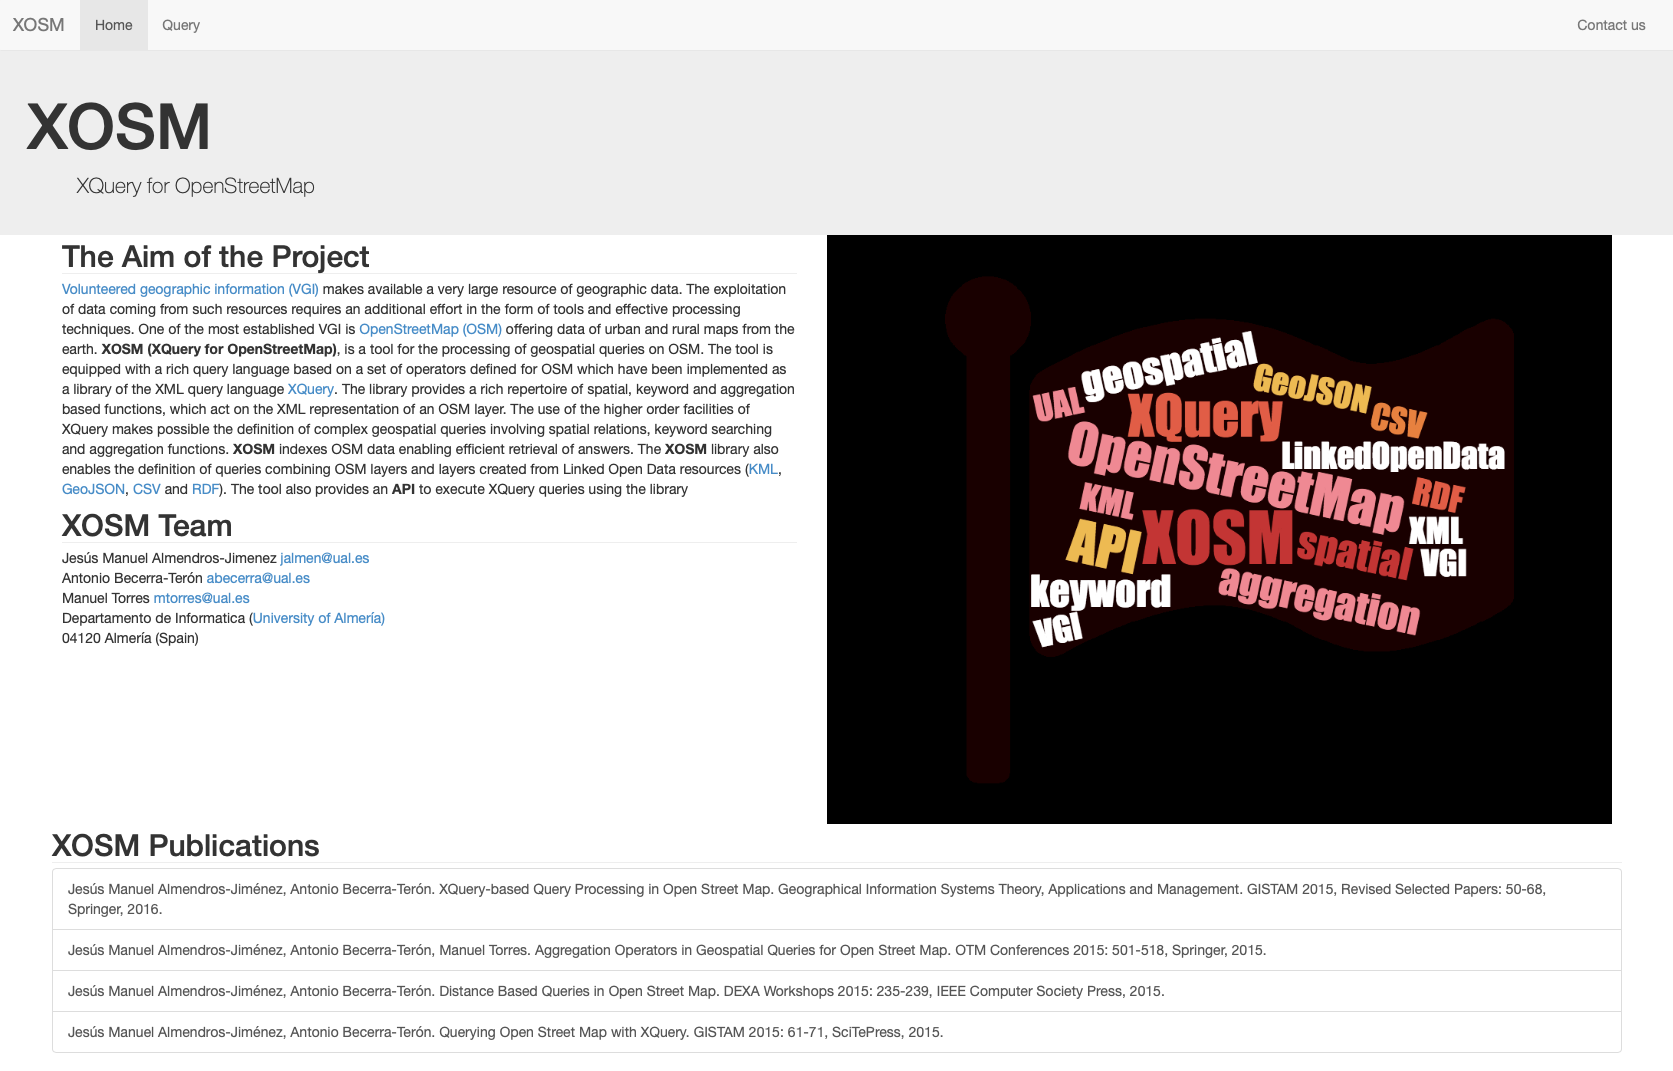
\includegraphics[width=0.7\linewidth]{imagenes/capitulo6/1}
	\caption{}
	\label{fig:1-6}
\end{figure}
\begin{figure}[H]
	\centering
	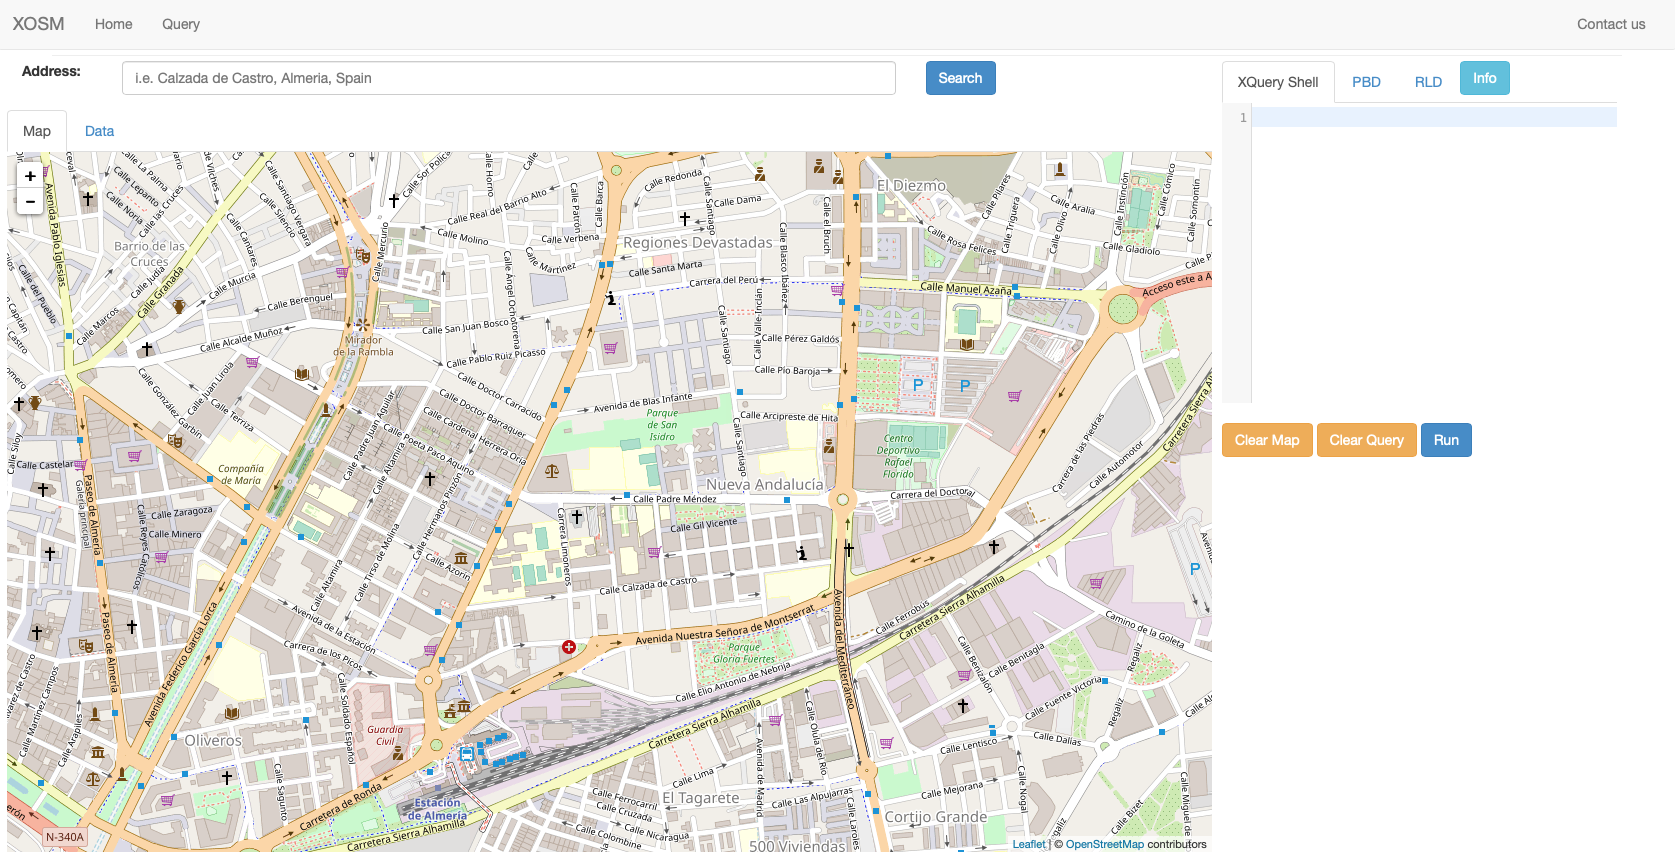
\includegraphics[width=0.7\linewidth]{imagenes/capitulo6/2}
	\caption{}
	\label{fig:2-6}
\end{figure}

\begin{figure}
	\centering
	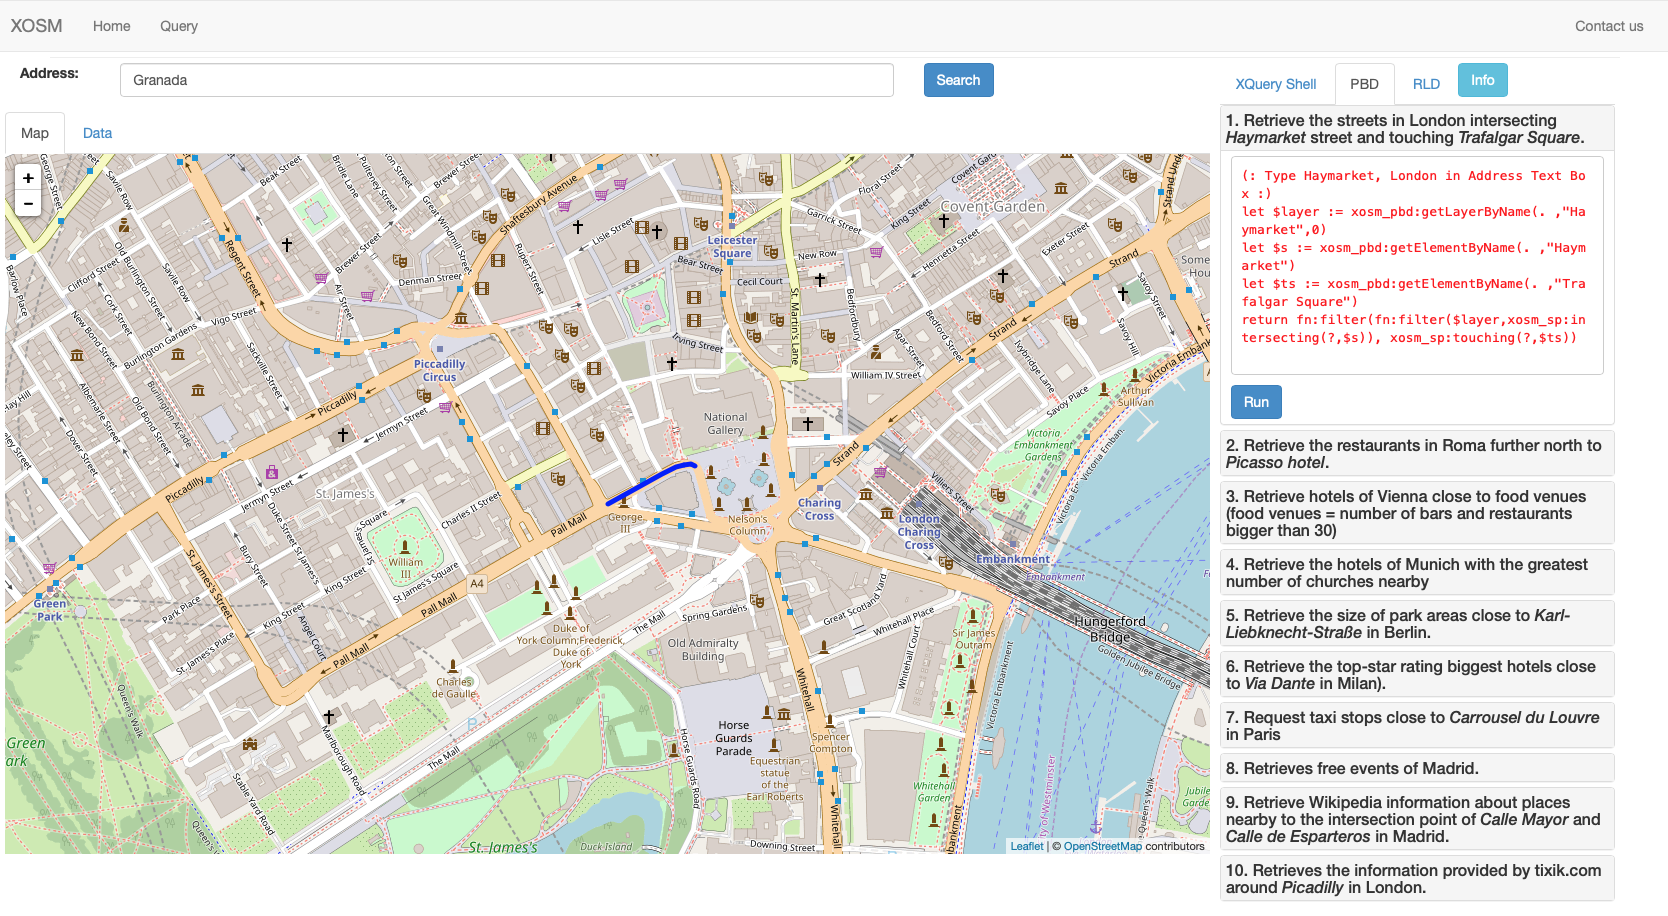
\includegraphics[width=0.7\linewidth]{imagenes/capitulo6/3}
	\caption{}
	\label{fig:3-6}
\end{figure}


Y como se observa este TFM se mantiene en la línea de estos proyectos.

\section{Trabajo futuro}

Durante la realización de este TFM se han encontrado temas, ejemplos o aplicaciones bastantes relacionados pero que no se han estudiado en el mismo, por este motivo, comentaremos algunos aspectos a profundizar en el futuro:

\begin{enumerate}
	
	\item Crear una plataforma parecida a la mostrada en las figuras anteriores, en donde a partir de la salida de la consulta que se haga, obtener el GID ubicado en el mapa.
	
	%\item Generar modelos para obtener la temperatura de una superficie a partir de la altitud y la localización del territorio.
	%\item Realizar un estudio con la función $terrain$ de R para la rugosidad del terreno, ya que dicha función no sólo permite obtener la pendiente y la orientación, sino otras variables cartográficas.
	%\item Ampliar el paquete desarrollado para facilitar este tipo de análisis, así como, aumentar el volumen de datos cargados en la misma, centrándonos en los MDT de España.
\end{enumerate}

%Adicionalmente, considero que este tema y el enfoque que le he dado puede tener interés para el público en general por lo que valoro la posibilidad de darle más difusión al trabajo.



